\documentclass[UTF8,12pt]{article}

\RequirePackage{geometry}   %页面设置
\RequirePackage{titlesec} %设置标题
\RequirePackage{fancyhdr} %定制页眉页脚
\usepackage[backend=biber,style=gb7714-2015ms,gbstyle=false]{biblatex}
\usepackage{ctex}
\usepackage{amsmath,amssymb}
\usepackage{graphicx}
\usepackage{listings}
\usepackage{color,xcolor}
\usepackage{authblk}
\usepackage{float}
\usepackage{wrapfig}
\usepackage{caption,subcaption}
\usepackage{tabularx,multirow,makecell,booktabs} 
\usepackage{framed}
\usepackage{fontspec}
\usepackage[titles]{tocloft}
\usepackage[hidelinks]{hyperref}
\usepackage{accsupp}

\linespread{1.5} \selectfont
\geometry{top=1in,bottom=1in,left=1in,right=1in}  %页面设置
%\setcounter{secnumdepth}{2}
\pagestyle{fancy} %页眉
\fancyhf{}
\fancyfoot[C]{\thepage}  
\fancyhead[C]{\slshape \leftmark}

\providecommand\Ket[1]{\left|\right. #1 \left.\right\rangle}
\providecommand\Bra[1]{\left\langle\right. #1 \left.\right|}

\providecommand\Bracket[2]{\left\langle #1 \big| #2 \right\rangle}
\providecommand\BraCket[3]{\left\langle #1 \big| #2 \big| #3 \right\rangle}
\providecommand\dual{\stackrel{DC}{\longleftrightarrow}}

\newenvironment{ale}{\begin{equation}\nonumber\begin{aligned}}{\end{aligned}\end{equation}}

\newcounter{partcount}
\setcounter{partcount}{1}
\titleformat{\part}{\centering\Large\bfseries}{第\zhnumber{\thepartcount}部分\stepcounter{partcount}}{1em}{}
\renewcommand{\thepart}{\chinese{part}}
\renewcommand{\thesection}{\Roman{section}}
\numberwithin{equation}{subsection}
\titleformat{\section}[frame]{\normalfont\large\bfseries\filright}{\fbox{\itshape\thesection}}{1em}{}

\setlength{\cftsecnumwidth}{2em}
\titleformat{\subsection}[block]{\normalfont\bfseries\filright}{\fbox{\itshape\thesubsection}}{1em}{}

\newcommand{\HRule}{\rule{\linewidth}{0.5mm}}

\definecolor{commentcode}{rgb}{0.4317,0.6667,0.3686}
\definecolor{codegray}{rgb}{0.6353,0.6353,0.6353}
\definecolor{maincode}{rgb}{0.3059,0.3059,0.3059}
\definecolor{keycode}{rgb}{0.3725,0.3725,0.9529}
\definecolor{backcolour}{rgb}{1,1,0.8784}
\definecolor{rulesepcolor}{rgb}{0.7843,0.7843,0.7559}
\definecolor{shadecolor}{rgb}{0.9686,0.9216,0.9216}%{gray}{0.95}

\providecommand{\empB}[1]{\textcolor{blue}{#1}}
\providecommand{\empR}[1]{\textcolor{red}{#1}}
\providecommand{\sumL}{\sum\limits}
\providecommand{\comment}[1]{\textcolor{commentcode}{#1}}
\newfontfamily\dejavu{DejaVu Sans Mono}
\newcommand\emptyaccsupp[1]{\BeginAccSupp{ActualText={}}#1\EndAccSupp{}}
\lstset{
	numbers=left,
	numbersep=5pt,
	tabsize=4,
	showstringspaces=false,
	numberstyle=\tiny\color{codegray}\emptyaccsupp,
	keywordstyle=\color{keycode},
	commentstyle=\color{commentcode},
	basicstyle=\footnotesize\dejavu\color{maincode},
	frame=shadowbox,
	rulesepcolor=\color{rulesepcolor},
	backgroundcolor=\color{backcolour},
	escapeinside={``},
	extendedchars=true,
	breaklines,
	language=[GNU]C++
}

\addbibresource{ref.bib}%references

\begin{document}
	\begin{titlepage}
		\begin{center}    
			\HRule \\[0.4cm]
			{ \huge \emph {从电子自旋窥见量子力学}}\\[0.4cm]%title
			\rule{\linewidth}{0.2mm} \\[1.5cm]
			
			\begin{minipage}{0.4\textwidth}
				\begin{flushleft} \large
				\end{flushleft}
			\end{minipage}
			\begin{minipage}{0.4\textwidth}
				\begin{flushright} \large
					%institute
					\Large 荒原%authur
				\end{flushright}
			\end{minipage}
			\vfill
			{\large \today}
		\end{center}
	\end{titlepage}
	\clearpage
	\tableofcontents
	\clearpage
	\part{理论简介}
	\section{引言}
	\subsection{量子力学的引入}
	量子力学学习入门大多数起于对黑体辐射中“紫外灾难”的解释。由于卢瑟福提出的原子行星轨道模型并不能用于解释原子的稳定性、化学结构等,玻尔通过构建量子化条件提出了玻尔模型。而在1925年,薛定谔写出了量子力学的基础方程之一,即薛定谔方程\footnote{很多教材会把该方程写为$\hat H\Psi=i\hbar \frac{\partial}{\partial t}\Psi$,而在选取合适的单位制下可以认为$\hbar=1$,下文不再特殊说明。}
	\begin{snugshade}
		\begin{equation}
			\hat H\Psi=i\frac{\partial}{\partial t}\Psi
			\label{Schroedinger}
		\end{equation}
	\end{snugshade}
		
	如果在式\ref{Schroedinger}中$\hat H$不显含时,式\ref{Schroedinger}可以分离变量得到定态薛定谔方程。此时构造$\hat H$来求得定态薛定谔方程的解,即可解释很多重要的物理现象。
	
	在1921至1922年间德国物理学家奥托·施特恩和瓦尔特·格拉赫完成了著名的“施特恩-格拉赫实验”(以下简称“SG实验”)以证实原子角动量量子化。在银原子的SG实验中,由于银原子只有一个价电子,忽略原子实的角动量变化,原子的角动量变化只体现在价电子的角动量变化上。银原子的SG实验体现了电子自旋的特殊性质,而该特殊性质并没有经典的宏观物理性质对应,是最能体现量子性质的现象之一。本文的主要参考教材\parencite{sakurai1995modern}便以此为切入点,从矩阵的角度来对量子力学进行展开阐释。
	\newpage
	\subsection{施特恩-格拉赫实验}
	\subsubsection{银原子的SG实验}
	\begin{figure}[H]
		\centering
		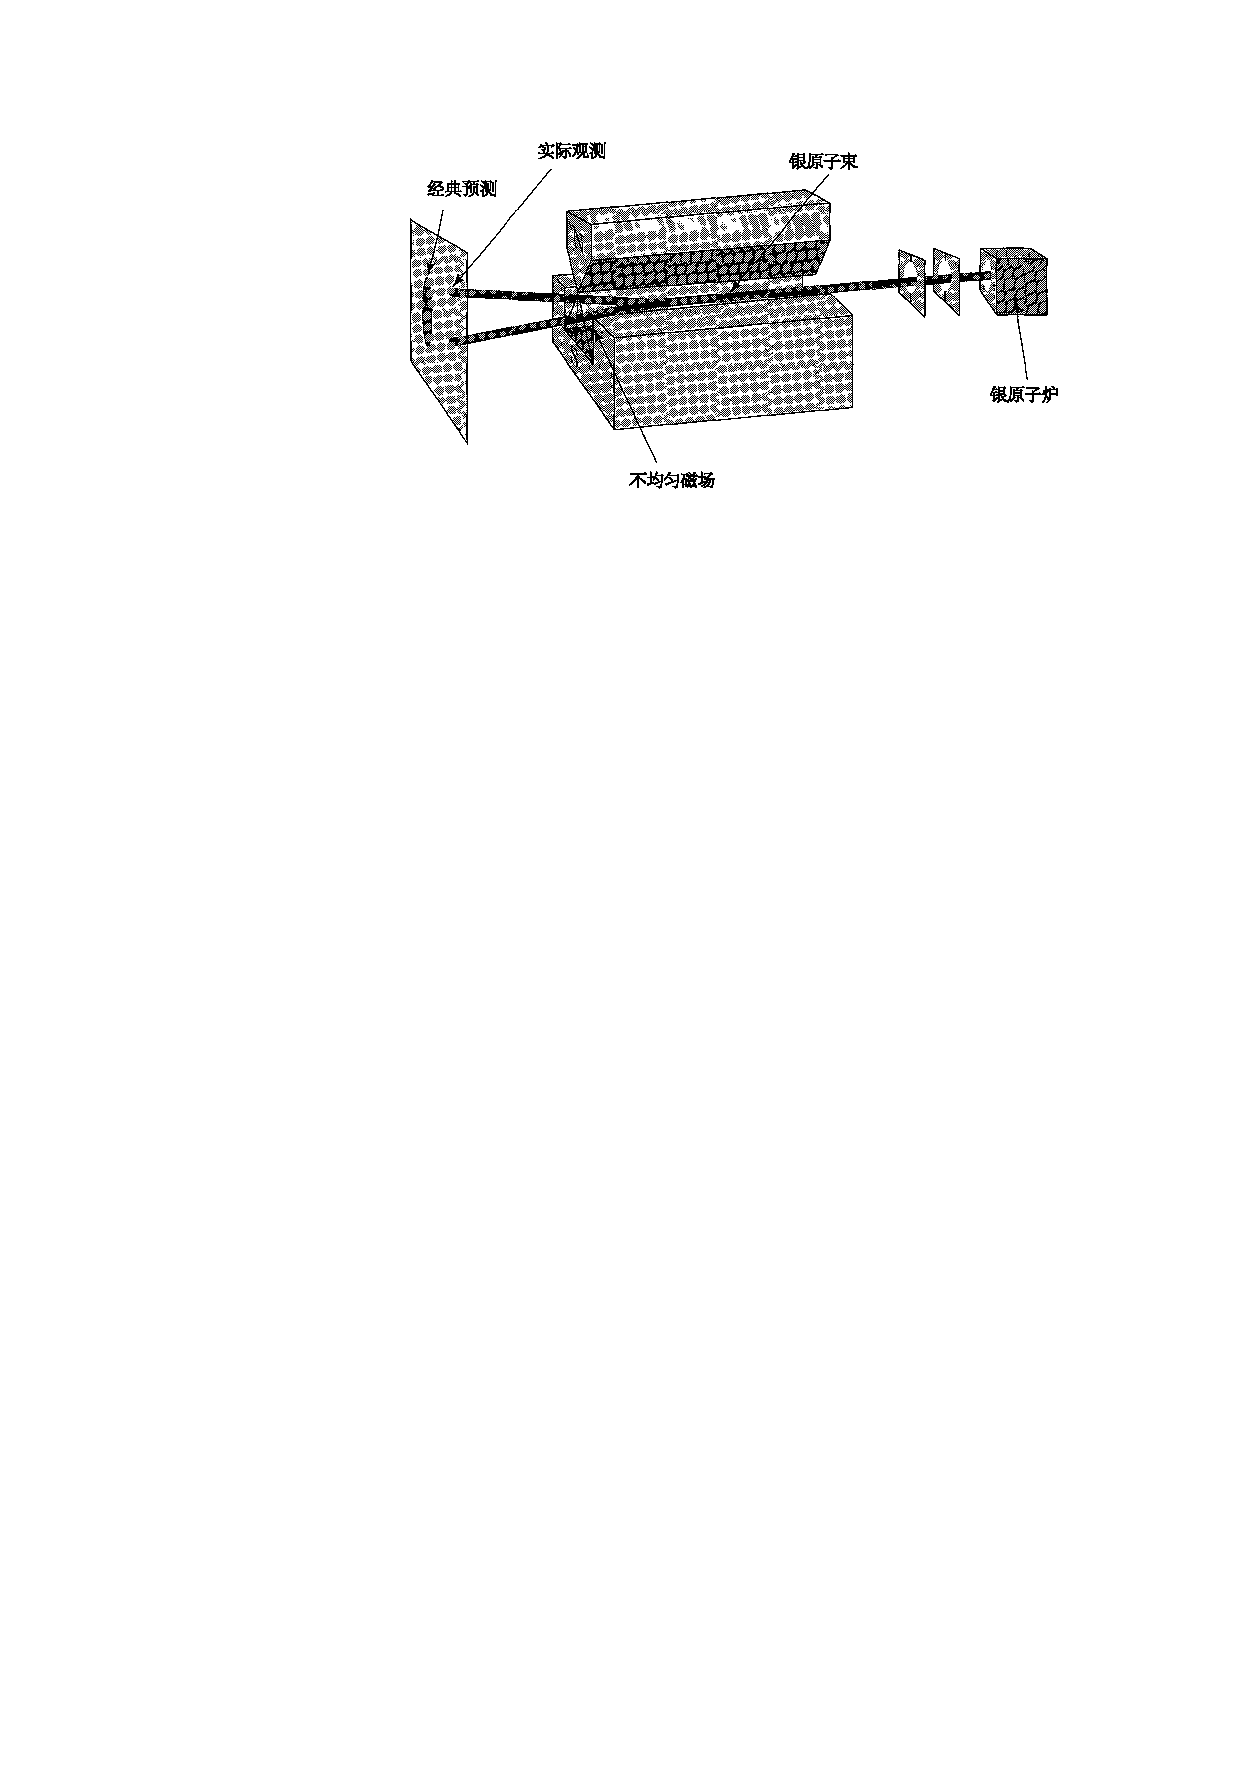
\includegraphics[width=0.4\linewidth]{SGe.pdf}
		\caption{银原子SG实验装置图}
	\end{figure}
	
	银原子在不均匀的磁场作用下被等分成了两束,若磁场梯度的方向沿$\hat z$,记磁场作用为$\mathcal S_z$,两束银原子分别用$\Ket{\mathcal S_z;\pm}$来表示\footnote{这里采用的符号为狄拉克符号,稍后将给出更为符合量子力学规范的定义与用法。},\empR{以后约定$\Ket{\pm}=\Ket{\mathcal S_z;\pm}$}。
	
	\subsubsection{序列的银原子SG实验}
	
	当磁场作用为$\mathcal S_x$时,银原子同样可以等分为$\Ket{\mathcal S_x;\pm}$两束(取$\hat y$方向为原子束的横向运动方向,这个方向上原子束做匀速直线运动)。用屏阻挡$\Ket{\mathcal S_x,-}$,使$\Ket{\mathcal S_x,+}$的银原子再经过$\mathcal S_z$作用,最终得到$\Ket{\pm}$两束银原子。这似乎给出一束银原子中“含有”四个“分量”的结论,但这个结论无法解释以下现象
	\begin{figure}[H]
		\centering
		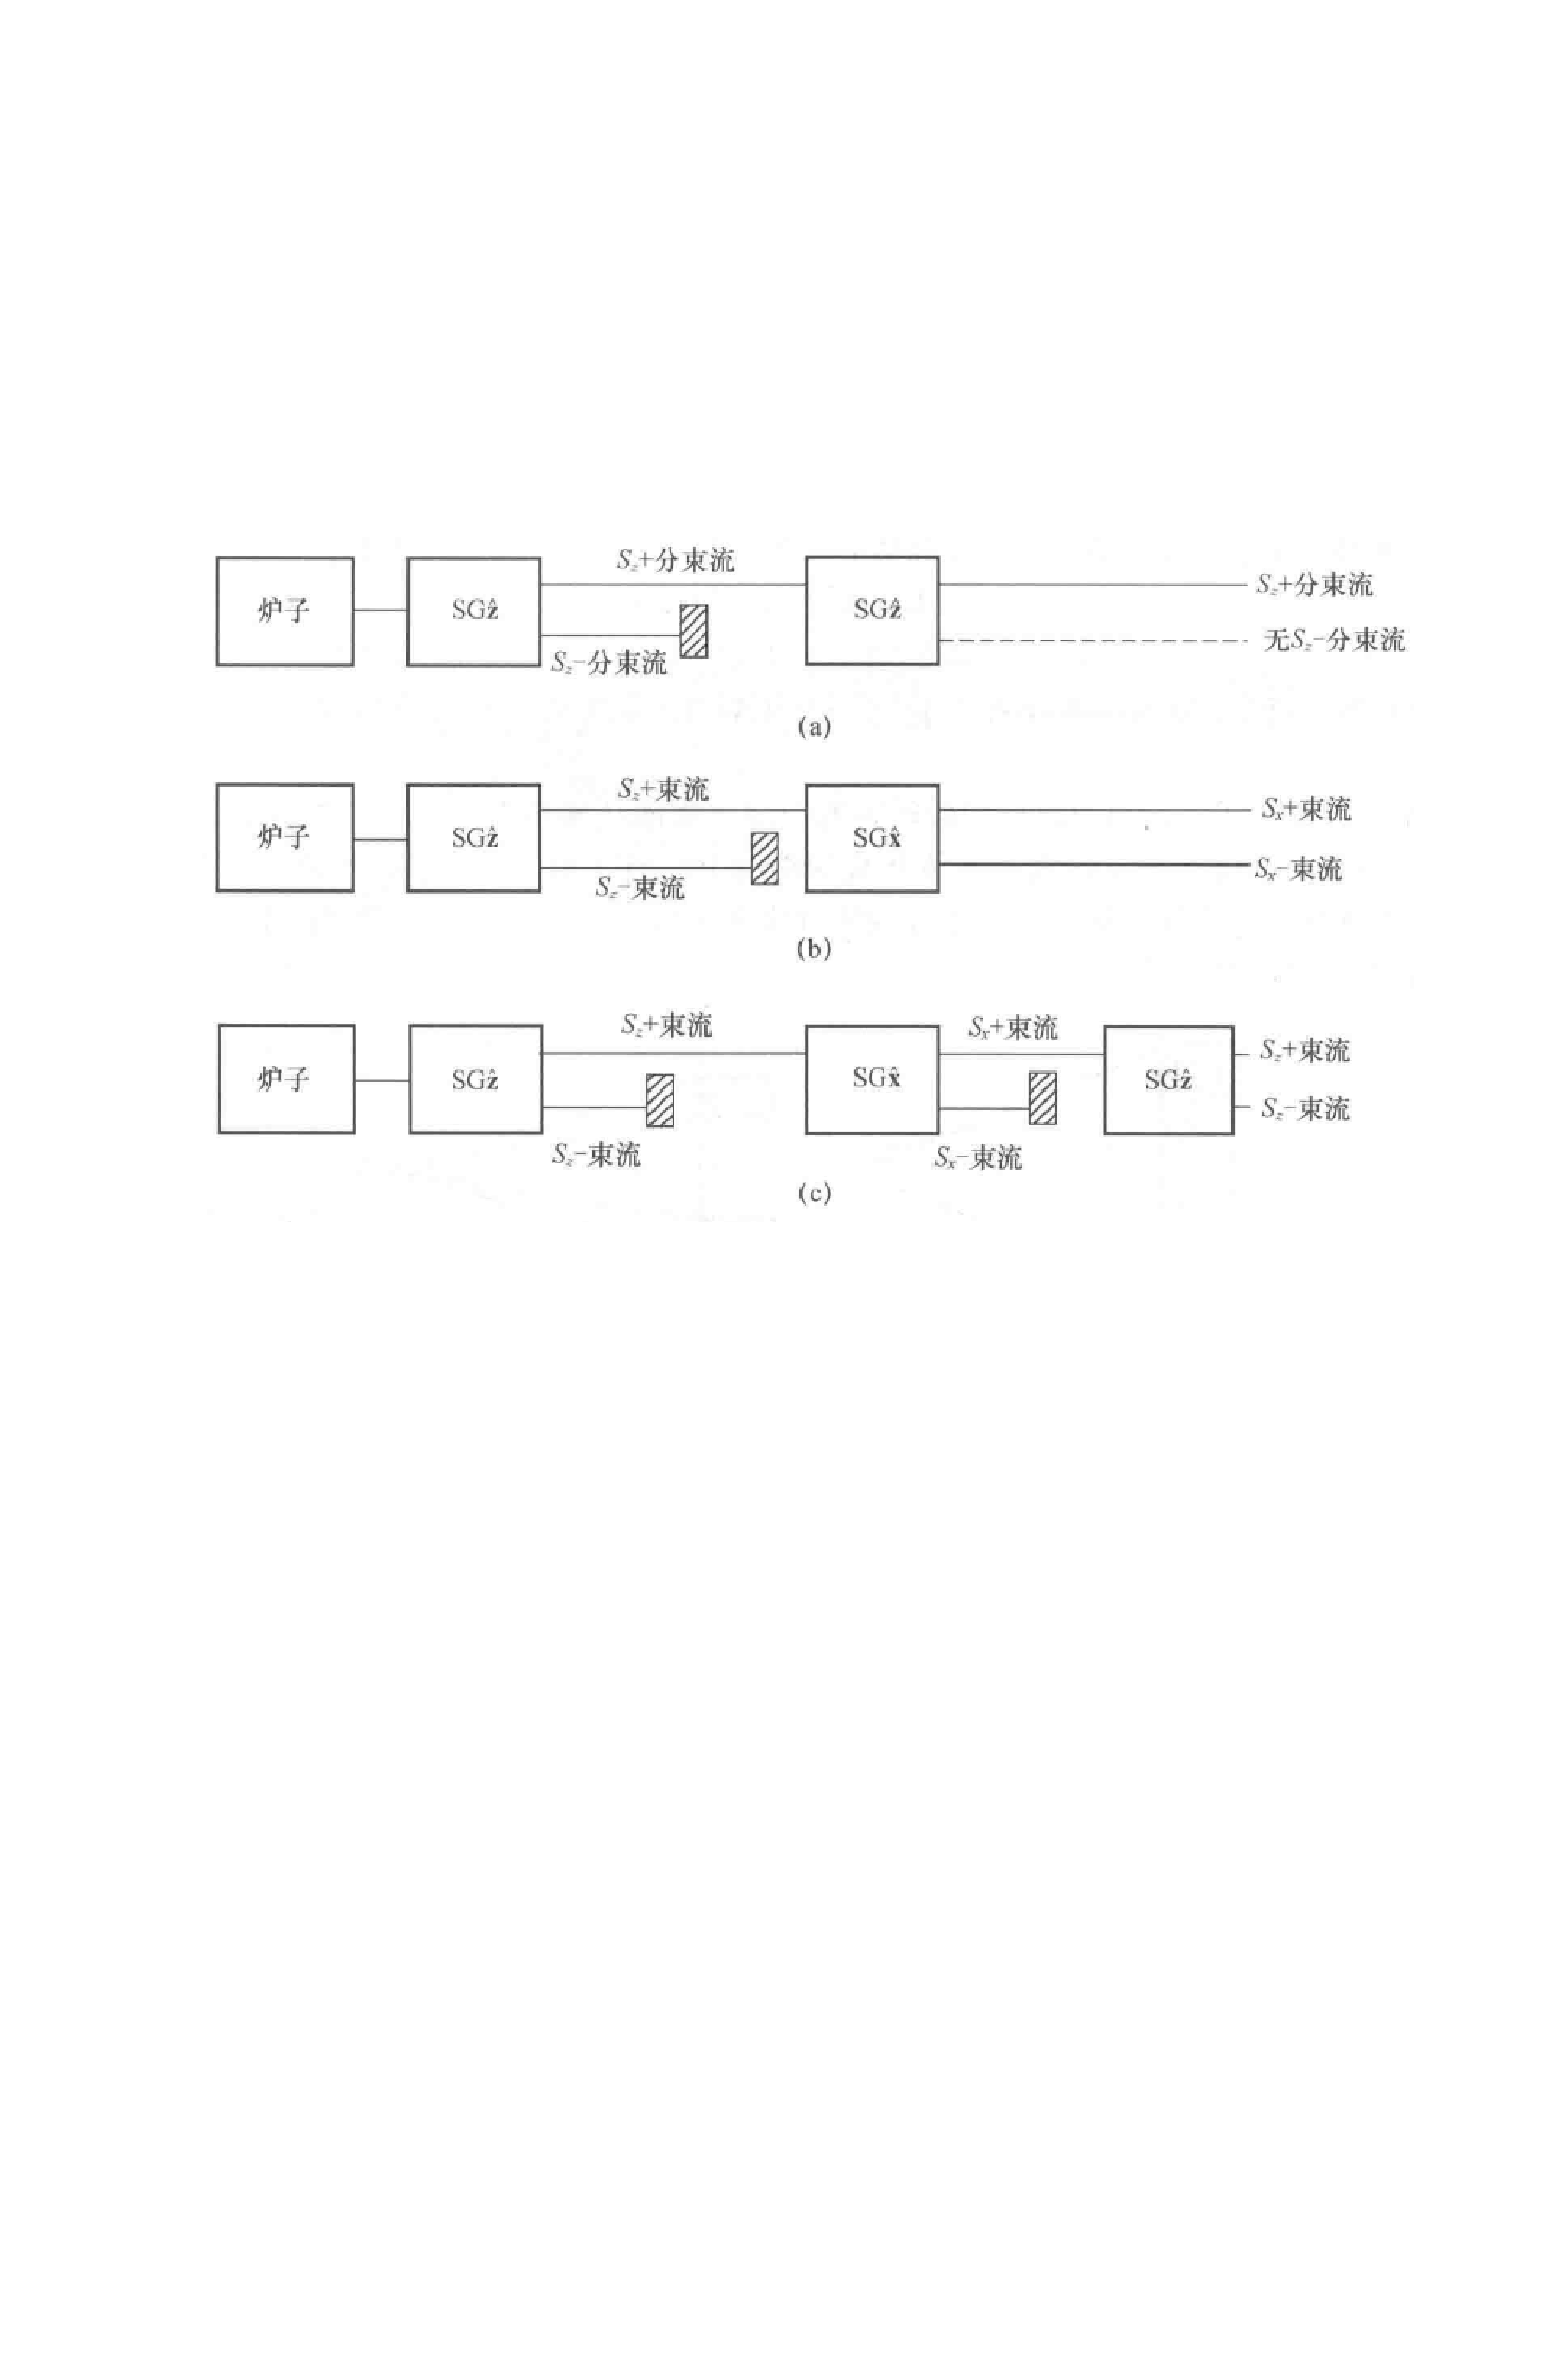
\includegraphics[width=0.6\linewidth]{sSGe.pdf}
		\caption{序列的银原子SG实验示意图}
		\label{sSGe}
	\end{figure}
	
	在图\ref{sSGe}.(c)中我们发现在第一次$\mathcal S_z$作用后我们已经用屏将$\Ket{-}$完全阻隔,结果中却出现了$\Ket{-}$分量。这表明图\ref{sSGe}.(c)中的仪器SG$\hat x$破坏了前一个仪器作用的信息。
	
	\subsubsection{序列的银原子SG实验与琼斯矩阵的类比}
	
	对于一束沿$\hat y$方向传播的线偏振光,我们可以构造其琼斯矢量
	\begin{ale}
		 E=\begin{bmatrix}
			\cos \alpha\\
			\sin \alpha
		\end{bmatrix},(0\leq\alpha\leq\frac{\pi}{2})
	\end{ale}

	然后让该偏振光依次经过透光轴沿$\hat x$方向、与$\hat x$夹$45^\circ$方向以及$\hat z$方向的偏振片,琼斯矩阵分别为
	\begin{ale}
		 J_x=\begin{bmatrix}
			1& 0\\
			0& 0
		\end{bmatrix},
		J_{xz}=
		\begin{bmatrix}
			\frac{1}{\sqrt{2}}& \frac{1}{\sqrt{2}}\\
			\frac{1}{\sqrt{2}}& \frac{1}{\sqrt{2}}
		\end{bmatrix},
		J_z=\begin{bmatrix}
			0& 0\\
			0& 1
		\end{bmatrix}
	\end{ale}

	作用的结果为\begin{ale}
		E' = J_zJ_{xz}J_xE=\begin{bmatrix}
			0\\
			\frac{\cos\alpha}{\sqrt{2}}
		\end{bmatrix}
	\end{ale}

	结论指出当$\alpha\not=\frac{\pi}{2}$时,$J_{xz}$会破坏$J_x$作用后的偏振信息,这与序列的银原子SG实验很类似。
	
	引入复数后,琼斯矩阵与琼斯矢量也可以用来描述光的相位信息,进而描述圆偏振光,这与后文会介绍的泡利矩阵高度类似。
	\section{基本概念}
	\subsection{右矢、左矢与算子}
	\begin{itemize}
		\item 右矢
		
		在量子力学里,我们对\empR{物理态}进行研究,而这些物理态都是存在于一个希尔伯特空间即\empR{右矢空间}里的,按保罗·狄拉克的建议,所有的物理态都被写为狄拉克符号下的\empR{右矢(ket)},即用\empB{$\Ket{\alpha}$}来表示矢量。
		
		\item 左矢与内积
		
		由线性代数的知识我们定义右矢的对偶矢量\empR{左矢(bra)},由左矢构成的空间为\empR{左矢空间},$c_\alpha\Ket{\alpha}$的左矢表达为$$c_\alpha\Ket{\alpha}\dual\empR{c^*_\alpha}\empB{\Bra{\alpha}},\text{($c_\alpha$与$c^*_\alpha$为共轭复数)}$$
		
		由左矢可以定义\empR{内积(inner product)~~\footnote{这个符号也被称为bracket,即bra(左矢)~c(column代表中间的|)~ket(右矢)。}$\Bracket{\beta}{\alpha}$}
		
		对于内积我们还有两条假设
		\begin{enumerate}
			\item $\Bracket{\beta}{\alpha}=\Bracket{\alpha}{\beta}^*$
			\item $\Bracket{\alpha}{\alpha}\geq0$,当且仅当$\Ket{\alpha}$为零右矢的时候等号成立。
			
			依此可以定义$\Ket{\alpha}$的模为$\sqrt{\Bracket{\alpha}{\alpha}}$,且可以得到非零右矢的归一化形式
			$$\Ket{\tilde\alpha}=\frac{\Ket\alpha}{\sqrt{\Bracket{\alpha}{\alpha}}}$$
		\end{enumerate}
	
	当$\Ket{\beta}\not = \Ket{\alpha}$且$\Bracket{\beta}{\alpha} =\Bracket{\alpha}{\beta}^*=0$,则定义$\Ket{\beta}$与$\Ket{\alpha}$\empR{正交}。
		
		\item 算子
		
		位置、动量以及自旋等被称为\empR{可观测量},可用所涉矢量空间的\empR{算子}来表示\footnote{部分算子由经典力学中的物理量如位置、动量“升格”得到,而自旋算子的特殊性在于其并没有经典物理量对应。}。算子从左侧作用到右矢上,作用结果仍是一个右矢,如算子\empB{$\mathcal A$}作用于右矢$\Ket{\alpha}$上表达为
		$$
			\mathcal A(\Ket{\alpha})=\mathcal A\Ket{\alpha}=\Ket{\bar{\alpha}}
		$$
		
		本文中所有算子都是线性算子,可以定义相等,对加法满足交换律、结合律,对乘法满足结合律但不满足交换律。
		
		算子从右侧作用到左矢上
		$$
			(\Ket{\beta})\mathcal B=\Bra{\beta}\mathcal B=\langle\bar{\beta}|
		$$
		
		从左矢与右矢的对偶关系可以得到$$\mathcal X\Ket{\alpha}\dual\Bra{\alpha}\empR{\mathcal X^\dagger}$$
		
		其中$\mathcal X^\dagger$为$\mathcal X$的\empR{伴算子},满足性质$(\mathcal{XY})^\dagger=\mathcal Y^\dagger \mathcal X^\dagger$。
		
		对于满足$$\empR{\mathcal X=\mathcal X^\dagger}$$的算子被称为\empR{自伴算子},有穷维内积空间上的自伴算子也被称为\empB{厄米算子},本文暂不涉及无穷维内积空间,以下讨论均使用厄米算子。
		
	\end{itemize}
	\subsection{结合公理与外积}
	
	狄拉克认为只要合理规定左矢、右矢与算子之间“乘法”的结合性,这种结合性就可以普遍适用,这被称为\empR{结合公理}。
	
	\begin{itemize}
		\item 外积
		
		右矢可以“乘以”左矢,即可以存在
		\begin{subequations}
			\begin{align}
				\mathcal Z &= \Ket{\alpha}\Bra{\beta}\label{o}\\
				\mathcal Z^\dagger &= \Ket{\beta}\Bra{\alpha}\label{od}
			\end{align}
		\end{subequations}
		
		可以验证式\ref{o}与式\ref{od}满足算子的运算律,因此这种假定是合理的,式\ref{o}即$\Ket{\alpha}$与$\Bra{\beta}$的\empR{外积(outter product)}。
		\item 简化书写
		
		结合公理给出$$\Bra{\beta}(\mathcal X\Ket{\alpha})=(\Bra \beta \mathcal X)\Ket{\alpha}=\BraCket{\beta}{\mathcal X}{\alpha}$$
		
		以及$$\BraCket{\alpha}{\mathcal X^\dagger}{\beta}=\BraCket{\beta}{\mathcal X}{\alpha}^*$$
	\end{itemize}
	\subsection{厄米算子的本征值和矩阵表示}
	\subsubsection{厄米算子的本征值}
	厄米算子是量子力学中的最重要的算子,由线性代数的结论,厄米算子的本征值一定是实数,且属于不同本征值的本征右矢是正交的,即满足
	\begin{snugshade}
		\begin{equation}
			\Bracket{\alpha^i}{\alpha^j}=\delta_{ij}
			\label{orth}
		\end{equation}
	\end{snugshade}

	在厄米算子的本征值\empR{不出现简并}时,不同本征值的本征右矢可以组成完备归一的基右矢即$\{\Ket{\alpha^i}\}$。任意右矢可以表示为基右矢的线性组合\begin{equation}
		\Ket{\alpha}=\sumL_ic_i\Ket{\alpha^i}
		\label{li}
	\end{equation}
	
	由式\ref{orth}可以得到系数的表达式为\begin{equation}
		c_i=\Bracket{\alpha^i}{\alpha}
		\label{coef}
	\end{equation}

	若按照量子力学的要求认为态$\Ket{\alpha}$是归一化的,即满足
	\begin{snugshade}
		\begin{equation}
			\Bracket{\alpha}{\alpha} = \sumL_i|\Bracket{\alpha^i}{\alpha}|^2=\sumL_i |c_i|^2=1
			\label{norm}
		\end{equation}
	\end{snugshade}
	
	将式\ref{coef}和式\ref{norm}带入式\ref{li}可以得到投影算符\begin{equation}
		\Lambda_i=\Ket{\alpha^i}\Bra{\alpha^i}
		\label{project}
	\end{equation}

	以及\empR{单位算符}
	\begin{snugshade}
		\empR{\begin{equation}
				\mathcal I=\sumL_i\Lambda_i=\sumL_i\Ket{\alpha^i}\Bra{\alpha^i}
		\end{equation}}
	\end{snugshade}
	\subsubsection{矩阵表示}
	对于任意厄米算子$\mathcal A$,总可以进行如下计算
	\begin{equation}
		\begin{aligned}
			\mathcal A &= \mathcal I\cdot \mathcal A\cdot \mathcal I\\
			  &= \sumL_i\sumL_j\Ket{\alpha^i}\Bra{\alpha^i}\mathcal A\Ket{\alpha^j}\Bra{\alpha^j}\\
			  &=\begin{bmatrix}
			  	\Ket{\alpha^1}&\cdots&\Ket{\alpha^i}&\cdots
			  \end{bmatrix}\empR{\begin{bmatrix}
			  \BraCket{\alpha^1}{\mathcal A}{\alpha^1}&\cdots&\BraCket{\alpha^1}{\mathcal A}{\alpha^i}&\cdots\\
			  \vdots&\ddots&\vdots&\\
			  \BraCket{\alpha^i}{\mathcal A}{\alpha^1}&\cdots&\BraCket{\alpha^i}{\mathcal A}{\alpha^i}\\
			  \vdots&&&\ddots
		  \end{bmatrix}}\begin{bmatrix}
	  		\Bra{\alpha^1}\\
  			\vdots\\
			\Bra{\alpha^i}\\
			\vdots
			\end{bmatrix}
		\end{aligned}
	\label{matrixO}
	\end{equation}
	
	由式\ref{matrixO}可以得到算子$\mathcal A$的\empR{矩阵表示$A$}\begin{snugshade}
		\begin{equation}
			\begin{aligned}
				A = \begin{bmatrix}
					\BraCket{\alpha^1}{\mathcal A}{\alpha^1}&\cdots&\BraCket{\alpha^1}{\mathcal A}{\alpha^i}&\cdots\\
					\vdots&\ddots&\vdots&\\
					\BraCket{\alpha^i}{\mathcal A}{\alpha^1}&\cdots&\BraCket{\alpha^i}{\mathcal A}{\alpha^i}\\
					\vdots&&&\ddots
				\end{bmatrix}
			\end{aligned}
			\label{matrix}
		\end{equation}
	\end{snugshade}

	很容易证明厄米算子的矩阵表示一定是\empB{厄米矩阵}。

	这样,我们建立了厄米算子和厄米矩阵之间的同构关系,而右矢也可以建立与列向量之间的对应关系。而线性代数给出的结论是,\empR{厄米矩阵一定可以通过酉矩阵进行相似对角化。}在计算中,求算子的本征值被转化为了求矩阵的本征值问题。
	\subsection{对狄拉克符号的评述}
	\subsubsection{物理意义}
	从线性代数的角度出发,用狄拉克符号表示出的右矢$\Ket{\psi}$与欧氏空间内的空间向量$\vec r$本质上是一致的。线性算子$\mathcal A$对右矢的作用本质上也是向量的线性运算。
	
	在物理上,右矢表示抽象的物理态,算子表示对物理态的测量。量子力学中最重要的厄米算子之一就是哈密顿算子$\mathcal H$,将哈密顿算子作用于物理态上可以得到哈密顿算子的\empR{本征值}与\empR{本征态}。不含时哈密顿算子的本征值即为对应物理态的\empB{能量}。
	\subsubsection{态与波函数的联系}
	算子的本征值可以是连续的,如规定坐标算子$\mathcal X$的本征值与本征态如下$$\mathcal X\Ket{x} = x\Ket{x}$$
	
	正交关系可以推广为$$\Bracket{x}{x'}=\delta(x-x')$$
	
	那么对态$\Ket{\alpha}$展开得到$$\Ket{\alpha} = \int dx\Ket{x}\Bracket{x}{\alpha}$$
	
	量子力学要求$\Bracket{\alpha}{\alpha}=1$
	
	可以认为$\psi_\alpha(x)=\Bracket{x}{\alpha}$,量子力学的归一化条件可以表述为
	\begin{snugshade}
		\begin{equation}
			\int |\psi_\alpha|^2=\int \psi^*_\alpha(x)\psi_\alpha(x)dx=1
			\label{normalize}
		\end{equation}
	\end{snugshade}
	
	这个结论可以推广到高维,在不同的空间坐标系下也适用,即
	\begin{snugshade}
		\begin{equation}
			\psi_\alpha(\boldsymbol{r}) = \Bracket{\boldsymbol{r}}{\alpha}
			\label{wave}
		\end{equation}
	\end{snugshade}
	
	对于定态,哈密顿算子作用于本征态上可以写为$$\mathcal H\Ket{\alpha} = E_\alpha\Ket{\alpha}$$
	
	两侧同时左乘$\Bra{\boldsymbol{r}}$得到$$\BraCket{\boldsymbol{r}}{\mathcal H}{\alpha}=E_\alpha\Bracket{\boldsymbol{r}}{\alpha}$$
	
	即式\ref{Schroedinger}$$\hat{H}\psi_\alpha=E_\alpha\psi_\alpha$$
	
	\section{角动量理论摘要}
	在量子力学中,角动量是一个更为抽象的概念。从宏观经典的视角切入,三维欧氏空间中的旋转有三个自由度,即绕$x,y,z$三根轴的旋转。有两个容易证明的结论,即
	\begin{enumerate}
		\item 绕三根坐标轴的旋转是对称的,不存在优先的旋转方向。
		\item 旋转的先后顺序是不能随意交换的。
	\end{enumerate}
	
	我们引入\empR{对易子$$[\mathcal A,\mathcal B]=\mathcal{AB}-\mathcal{BA}$$}
	
	来描述两个算子之间的对易关系。很明显$[\mathcal A,\mathcal B]=0$时,$\mathcal A,\mathcal B$两算子对易,由线性代数的结论可知,两算子对易意味着它们有相同的本征向量组,可以同时对角化。
	\subsection{角动量基本对易关系}
	经典力学下角动量的定义为$$\boldsymbol{L}=\boldsymbol{r}\times \boldsymbol{p}$$
	
	$\boldsymbol{L}$有三个分量即$$\boldsymbol{L}=[L_x~L_y~L_z]$$
	
	仿照经典力学的定义可以定义量子力学下的轨道角动量\begin{equation}
		\mathcal L = \mathcal R\times \mathcal P
		\label{orbit}
	\end{equation}
	
	其中$\mathcal R=[\mathcal X~\mathcal Y~\mathcal Z],\mathcal P=[-i\nabla_x~-i\nabla_y~-i\nabla_z]$
	
	利用列维-奇维塔符号\begin{equation}
		\nonumber
		\begin{aligned}
		\varepsilon_{ijk}=\begin{cases}
			1,&ijk\text{为偶排列}\\
			-1,&ijk\text{为奇排列}\\
			0,&ijk\text{中存在相等}
		\end{cases}
		\end{aligned}
	\end{equation}
	
	可以写出
	\begin{snugshade}
		\empR{\begin{equation}
				[\mathcal L_i,\mathcal L_j] = \footnote{\text{此处的i为虚数单位,下同。}}i\varepsilon_{ijk}\mathcal L_k
				\label{angularMomentum}
		\end{equation}}
	\end{snugshade}

	其实在量子力学中,三个满足如上关系的厄米算子都被称为角动量算子,这种关系被称为\empR{角动量基本对易关系}。
	
	角动量算子还满足雅可比恒等式,即$$[\mathcal L_x,[\mathcal L_y,\mathcal L_z]]+[\mathcal L_y,[\mathcal L_z,\mathcal L_x]]+[\mathcal L_z,[\mathcal L_x,\mathcal L_y]]=0$$
	\subsection{升降算子与本征右矢}
	对于满足基本对易关系的角动量组$\mathcal J=[\mathcal J_x~\mathcal J_y~\mathcal J_z]$,其具有一些普适的、与角动量具体形式无关的重要结论。
	
	虽然角动量算子的三个分量是对称的,在进行坐标变换的时候,我们会认为$\phi$角的旋转轴与$z$轴重合,并且在SG实验中,我们也认为以磁场梯度方向为$\hat z$方向为基础。因此我们对$\mathcal J_z$予以特殊的关注。而对$\mathcal J_x,\mathcal J_y$进行如下变换,定义\empR{升降算子}
	\begin{snugshade}
		\begin{align}
			\begin{cases}
				\mathcal J_+ = \mathcal J_x+i\mathcal J_y\\
				\mathcal J_- = \mathcal J_x-i\mathcal J_y
			\end{cases}
			\label{raiselower}
		\end{align}
	\end{snugshade}

	$\mathcal J_+,\mathcal J_-$二者都不是厄米算子,但是两者互为伴算子,且$\mathcal J_+\mathcal J_-,\mathcal J_-\mathcal J_+$均为厄米算子。且满足关系\begin{equation}
		[\mathcal J_+,\mathcal J_-] = \mathcal J_+\mathcal J_--\mathcal J_-\mathcal J_+=2\mathcal J_z
		\label{updown}
	\end{equation}
	
	定义角动量平方算子\begin{equation}
		\mathcal J^2 = \frac{1}{2}(\mathcal J_+\mathcal J_-+\mathcal J_-\mathcal J_+)+\mathcal J^2_z=\mathcal J^2_x+\mathcal J^2_y+\mathcal J^2_z
		\label{square}
	\end{equation}
	
	
	可以证明\empB{$$[\mathcal J^2,\mathcal J_z]=0$$}
	
	这意味着二者有共同的本征右矢组,由式\ref{square}可知,$\mathcal J^2$的本征值一定为非负数,所以可以设$\mathcal J^2$与$\mathcal J_z$的共同本征右矢为\empR{$\Ket{j,m},j\geq 0$},有
	\begin{snugshade}
		\begin{subequations}
			\begin{align}
				\mathcal J^2 \Ket{j,m}&=j(j+1)\Ket{j,m}\label{j}\\
				\mathcal J_z \Ket{j,m}&=m\Ket{j,m}\label{m}
			\end{align}
		\end{subequations}
	\end{snugshade}

	升降算子的“升降”二字体现在如下关系中
	\begin{snugshade}
		\begin{align}
			&[\mathcal J_z,\mathcal J_{\pm}] = \pm \mathcal J_{\pm}\label{raiselowerex}\\
			&\mathcal J_z\mathcal J_\pm = \mathcal J_\pm(\mathcal J_z\pm \mathcal I)\label{raiselowerexZ}
		\end{align}
	\end{snugshade}
	
	在式\ref{raiselowerexZ}两边同时右乘$\Ket{j,m}$得到
	\begin{align*}
		\mathcal J_z\empB{\mathcal J_\pm\Ket{j,m}} &= \mathcal J_\pm(\mathcal J_z\pm \mathcal I)\Ket{j,m}\\
						  &=(m\pm1)\mathcal J_\pm\Ket{j,m}\\
						  &=(m\pm1)\empB{\Ket{j,m\pm1}}
	\end{align*}
	
	上式表明升降算子可以将$\mathcal J_z$本征值为$m$的本征右矢变换为本征值为$m+1$的本征右矢。
	
	由式\ref{updown}和式\ref{square}可以得到如下关系\begin{subequations}
		\nonumber
		\begin{align}
			\mathcal J_+\mathcal J_-=\mathcal J^2-\mathcal J^2_z+\mathcal J_z\\
			\mathcal J_-\mathcal J_+=\mathcal J^2-\mathcal J^2_z-\mathcal J_z
		\end{align}
	\end{subequations}

	由本征右矢不为$0$可以得到
		\begin{subequations}
			\nonumber
			\begin{align}
				\Bracket{j,m-1}{j,m-1}=\BraCket{j,m}{J_+J_-}{j,m}=j(j+1)-m^2+m\geq0\\
				\Bracket{j,m+1}{j,m+1}=\BraCket{j,m}{J_-J_+}{j,m}=j(j+1)-m^2-m\geq0
			\end{align}
		\end{subequations}
	
	解得
	\begin{snugshade}
		\empB{\begin{equation}
				-j\leq m\leq j
				\label{fond}
		\end{equation}}
	\end{snugshade}
	
	\empB{$m$的最大值必然取$j$,否则有$j-1<m_{max}<j$使得$\Bracket{j,m+1}{j,m+1}<0$。同理,$m$的最小值必然取$-j$。此时有$$\mathcal J_\pm\Ket{j,\pm j}=0$$}
	
	因此我们得到$m_{max}-m_{min} = 2j = k,k\in \mathbb{N}$,即\empR{$j$一定为非负整数或者正半奇数,$m$仅且一定取遍$-j,-j+1,\dots,j$。}
	
	上述结论不涉及角动量算子的具体形式,为量子力学中角动量的普适结论,这也是量子力学中态是不连续的直接体现。
	\subsection{轨道角动量与球谐函数}
	量子力学的结论进一步指出,当$j$为非负整数时角动量是有经典力学的物理量对应的,式\ref{orbit}给出的轨道角动量$\mathcal L$即对应三维坐标空间中的旋转。在式\ref{j}与式\ref{m}两边同时乘以球坐标下的本征左矢可以得到\empR{球谐函数}
	\begin{equation}
		\nonumber
		\begin{aligned}
			&\begin{cases}
				\BraCket{\boldsymbol{r}}{\mathcal L^2}{l,m}&=l(l+1)\Bracket{\boldsymbol{r}}{l,m}\\
				\BraCket{\boldsymbol{r}}{\mathcal L_z}{l,m}&=m\Bracket{\boldsymbol{r}}{l,m}
			\end{cases}\\		
		&\hspace{13em}\Downarrow\\
		&\begin{cases}
			-\left[\frac{1}{\sin^2\theta}\frac{\partial^2}{\partial\varphi^2}+\frac{1}{\sin\theta}\frac{\partial}{\partial\theta}\left(\frac{1}{\sin\theta}\frac{\partial}{\partial\theta}\right)\right]Y^m_l(\theta,\varphi)=l(l+1)Y^m_l(\theta,\varphi)\\
			-i\frac{\partial}{\partial\varphi}Y^m_l(\theta,\varphi)=mY^m_l(\theta,\varphi)
		\end{cases}
		\end{aligned}
	\end{equation}
	
	当$j$取正半奇数时,$\mathcal J$为自旋角动量,没有经典力学的物理量对应,下一章会详细讨论。

\section{自旋$1/2$系统}
	\subsection{构造单自旋系统的角动量与泡利矩阵}
	我们在寻找算子的矩阵表示时发现式\ref{matrix}中的$$\BraCket{\alpha^i}{\mathcal A}{\alpha^j} = \alpha^j\delta_{ij}$$
	
	那么算子可以表示为\begin{equation}
		\mathcal A = \sumL_i\alpha_i\Ket{\alpha^i}\Bra{\alpha^i}=\sumL_i\alpha_i\Lambda_i
		\label{ei-projector}
	\end{equation}
	
	单自旋$\frac{1}{2}$系统的本征向量可以被表示为已归一化的$\Ket{\pm}$,可以构造单位算子$$\mathcal I = \Ket{+}\Bra{+}+\Ket{-}\Bra{-}$$
	
	由于需要满足\ref{ei-projector}要求,梯度沿$\hat z$方向的磁场作用可以构造为
		\begin{equation}
			\mathcal S_z = \frac{1}{2}\left(\Ket{+}\Bra{+}-\Ket{-}\Bra{-}\right)
			\label{Sz}
		\end{equation}
	
	同时构造升降算子
	\begin{snugshade}
	\begin{subequations}
		\begin{align}
			\mathcal S_+=\Ket{+}\Bra{-}\label{sUp}\\
			\mathcal S_-=\Ket{-}\Bra{+}\label{sDown}
		\end{align}
	\end{subequations}
	\end{snugshade}

	由图\ref{sSGe}.(b)可知
	\begin{equation}
		\begin{aligned}
			&|\Bracket{+}{\mathcal S_x;+}|^2+|\Bracket{-}{\mathcal S_x;+}|^2=1\\
			&|\Bracket{+}{\mathcal S_x;+}|^2=|\Bracket{-}{\mathcal S_x;+}|^2
		\end{aligned}
		\label{expectation}
	\end{equation}
	
	再由正交归一化条件构造\begin{align*}
		\Ket{\mathcal S_x;+} &= \frac{1}{\sqrt{2}}\left(\Ket{+}+e^{i\delta_1}\Ket{-}\right)\\
		\Ket{\mathcal S_x;-} &= \frac{1}{\sqrt{2}}\left(\Ket{+}-e^{i\delta_1}\Ket{-}\right)
	\end{align*}

	那么梯度沿$\hat x$方向的磁场作用可以写为\begin{equation}
		\mathcal S_x = \frac{1}{2}\left(e^{-i\delta_1}\Ket{+}\Bra{-}+e^{i\delta_1}\Ket{-}\Bra{+}\right)
		\label{Sx}
	\end{equation}

	同理可以构造\begin{align}
		&\Ket{\mathcal S_y;+} = \frac{1}{\sqrt{2}}\left(\Ket{+}+e^{i\delta_2}\Ket{-}\right)\notag\\
		&\Ket{\mathcal S_y;-} = \frac{1}{\sqrt{2}}\left(\Ket{+}-e^{i\delta_2}\Ket{-}\right)\notag\\
		&\mathcal S_y = \frac{1}{2}\left(e^{-i\delta_2}\Ket{+}\Bra{-}+e^{i\delta_2}\Ket{-}\Bra{+}\right)
		\label{Sy}
	\end{align}
	
	与式\ref{expectation}对比可以写出
	\begin{equation}
		\begin{aligned}
			&|\Bracket{\mathcal S_y;+}{\mathcal S_x;+}|^2+|\Bracket{\mathcal S_y;-}{\mathcal S_x;+}|^2=1\\
			&|\Bracket{\mathcal S_y;+}{\mathcal S_x;+}|^2=|\Bracket{\mathcal S_y;-}{\mathcal S_x;+}|^2
		\end{aligned}
	\end{equation}

	若取$\delta_1 = 0$,有$e^{i\delta_2}=\pm i$,在取定右手坐标系,同时要求式\ref{sUp}~\ref{sDown}满足式\ref{raiselower}定义时,取定$e^{i\delta_2}=i$。
	
	最终我们得到\empB{$\mathcal S=[\mathcal S_x~\mathcal S_y~\mathcal S_z]$}
	\begin{snugshade}
		\empB{\begin{equation}
			\begin{aligned}
				\mathcal S_x &= \frac{1}{2}\Big(\Ket{+}\Bra{-}+\Ket{-}\Bra{+}\Big)\\
				\mathcal S_y &= \frac{i}{2}\Big(-\Ket{+}\Bra{-}+\Ket{-}\Bra{+}\Big)\\
				\mathcal S_z &= \frac{1}{2}\Big(\Ket{+}\Bra{+}-\Ket{-}\Bra{-}\Big)
			\end{aligned}
			\label{spin}
		\end{equation}}
	\end{snugshade}

	以及升降算子
	
	\begin{snugshade}
		\empB{\begin{equation}
				\begin{aligned}
					\mathcal S_+=\mathcal S_x+i\mathcal S_y=\Ket{+}\Bra{-}\\
					\mathcal S_-=\mathcal S_x-i\mathcal S_y=\Ket{-}\Bra{+}
				\end{aligned}
				\label{raiselowerS}
		\end{equation}}
	\end{snugshade}
	
	$\mathcal S=[\mathcal S_x~\mathcal S_y~\mathcal S_z]$是厄米的,且满足角动量基本对易关系式\ref{angularMomentum},即$$[\mathcal S_i,\mathcal S_j] = i\varepsilon_{ijk}\mathcal S_k$$
	
	因此,$\mathcal S$即单自旋$\frac{1}{2}$系统的\empR{自旋角动量}。
	
	在$\mathcal S$的分量两边同时乘以单位算子,可以得到得到\empR{泡利矩阵}
	\begin{snugshade}
		\begin{equation}
				\begin{aligned}
					\sigma_x = \frac{1}{2}\begin{bmatrix}
						0&1\\
						1&0
					\end{bmatrix}~
					\sigma_y = \frac{1}{2}\begin{bmatrix}
						0&-i\\
						i&0
					\end{bmatrix}~
					\sigma_z = \frac{1}{2}\begin{bmatrix}
						1&0\\
						0&-1
					\end{bmatrix}
				\end{aligned}
				\label{PauliMatrix}
		\end{equation}
	\end{snugshade}
	\subsection{多自旋系统}
	\small
	\subsubsection*{\small{符号约定}}
	\emph{
	在讨论多自旋系统前先进行一个符号约定,在不至于引起混淆的情况下,下标$i$表示第$i$个角动量、态等,上标表示相应角动量、态等的分量。如$\mathcal S^z_2$表示作用于态$\Ket{\varPsi_2}$上的自旋角动量的$z$分量。}
	\normalsize
	\subsubsection{多自旋系统的右矢空间}
	在引入多个自旋相互用之后,可以认为每一个角动量算子都只作用在对应的态上,而不作用于其他的态,角动量的基本对易关系也可以表达为
	\begin{equation}
		[\mathcal S^i_m,\mathcal S^j_n]=i\varepsilon_{ijk}\delta_{mn}\mathcal S^k_m
		\label{exchange}
	\end{equation}
	
	上式表明了下标不同的$\mathcal S^z_i$之间是\empR{相容}的,这表明了它们有共同的本征右矢。即自旋角动量可以进行线性叠加,而叠加后的角动量作用的希尔伯特空间可以写成每个自旋态的直积\cite{Bose},即$$\Ket{\varPsi} = \Ket{\varPsi_1}\otimes\Ket{\varPsi_2}\otimes\dots\otimes\Ket{\varPsi_L}$$
	
	对于自旋和自旋角动量来说,本征向量组可以写为如下形式\begin{snugshade}
		\begin{equation}
			\begin{aligned}
				\text{共}2^L\text{个}\left\lbrace
				\begin{array}{ll}
					\Ket{\overbrace{++\cdots+}^{\text{共}L\text{个}}&}\\
					\Ket{++\cdots-&}\\
					\vdots&\\
					\Ket{--\cdots-&}
				\end{array}
				\right.
			\end{aligned}
			\label{ein}
		\end{equation}
	\end{snugshade}

	式\ref{ein}表明了随着自旋态的增多,用于描述自旋的本征向量是成指数规律增加的,这为与自旋相关的计算带来了不小的困难,这意味着我们需要寻求更多的物理关系来去除冗余的部分使得计算变得简化。
	\subsubsection{多自旋系统的角动量}
	多自旋系统的角动量可以表示为所有的自旋角动量的和,即
	\begin{equation}
			\nonumber
			\begin{aligned}
				\mathcal S^i =~ &\mathcal S^i_1\otimes \mathcal I_2\otimes\cdots\otimes \mathcal I_L\\
				+ &\mathcal I_1\otimes \mathcal S^i_2\otimes\cdots\otimes \mathcal I_L\\
				\vdots\\
				+ &\mathcal I_1\otimes \mathcal I_2\otimes\cdots\otimes \mathcal S^i_L
			\end{aligned}
	\end{equation}
	
	可以简化为
	\begin{snugshade}
		\empB{\begin{equation}
			\mathcal S^i = \sumL_m\mathcal S^i_m
			\label{multispin}
		\end{equation}}
	\end{snugshade}
	
	这种方式定义的角动量,结合\ref{exchange},是能够满足角动量基本对易关系,即式\ref{angularMomentum}的。
	
	升降算子的定义与式\ref{raiselowerS}一致,角动量平方算子的定义也与前文保持一致,即
	\begin{snugshade}
		\begin{equation}
			\mathcal S^2 = \frac{1}{2}(\mathcal S^+\mathcal S^-+\mathcal S^-\mathcal S^+)+(\mathcal S^z)^2
			\label{multisquare}
		\end{equation}
	\end{snugshade}

	也有
	\begin{snugshade}
		\begin{equation}
			[\mathcal S^2,\mathcal S^z]=0
			\label{multiSz}
		\end{equation}
	\end{snugshade}
	
	我们发现$\mathcal S^z\Ket{++\cdots+}=\frac{L}{2}\Ket{++\cdots+}$,表明$j=m_{max}=\frac{L}{2}$
	
	很明显$L$的奇偶性决定了系统的对称性,当$L$为偶数的时候,存在$m=0$的能量最低态,该系统为\empR{玻色子系统},后文将对一个玻色子系统进行简单的分析。
	
	当$L$为奇数的时候,系统能量最低态是二重简并的,且能量高于玻色子系统,此系统为\empR{费米子系统}。
	\newpage
	\part{玻色子系统计算实例}
	\section{引言}
		前文构建多自旋系统时,我们发现当需要考虑的自旋个数增多时,右矢空间的维度会与自旋个数成指数关系增加。而实际上在考虑两个自旋相互作用时,角动量算子对应的矩阵就已经是$4\times 4$的矩阵了,为此我们不得求助于计算机程序来解算或近似解算我们所需的数据。
		
		本部分将构建简化的一维海森堡模型,给出并简要分析由对称性所决定的简化方法。还将给出一个多自旋系统的数据存储方案,并给出一些数值计算结果。本部分的主要参考文献为\parencite{Bose},下文均为玻色子系统。
		
		笔者在测试时使用的编程语言为C++,测试环境为Ubuntu~20.04LTS下集成开发环境CLion~2021.1.3x64,编译器为GCC~9.3.0,科学计算模块为GSL-2.7。
		
		\newpage
	\section{简化的一维海森堡模型}
		\subsection{模型构建与分析}
		简化的一维海森堡模型只考虑相邻自旋的相互作用,且作用系数为$1$,开放边界条件\footnote{还可以考虑周期边界条件,即考虑最后一个自旋和第一个自旋相互作用,分析方法与开放边界条件一致。}。所以对于一维自旋$\frac{1}{2}$链,哈密顿算子写为如下形式
		\begin{snugshade}
			\begin{equation}
				\begin{aligned}
					\mathcal H &= \sumL^{L-1}_{i=1}\mathcal S_i\cdot \mathcal S_{i+1}\\
					&= \sumL^{L-1}_{i=1}\Big(\mathcal S^x_i\mathcal S^x_{i+1}+\mathcal S^y_i\mathcal S^y_{i+1}+\mathcal S^z_i\mathcal S^z_{i+1}\Big)\\
					&= \sumL^{L-1}_{i=1}\left[ \frac{1}{2}(\mathcal S^+_i\mathcal S^-_{i+1}+\mathcal S^-_i\mathcal S^+_{i+1})+\mathcal S^z_i\mathcal S^z_{i+1}\right]
				\end{aligned}
				\label{Hamiltonian}
			\end{equation}
		\end{snugshade}
		
	式\ref{Hamiltonian}中使用了升降算子,即式\ref{raiselowerS}来进行构造,这样做的好处是,哈密顿算子中的所有算子都是对$\mathcal S^z$的本征右矢定义的,而且不会引入虚数。由于构成$\mathcal H$的算子均是厄米算子,$\mathcal H$也是厄米算子。
	
	计算的任务是寻找哈密顿算子的本征值和本征态,本征态是系统可以稳定存在的态,而本征值系统处在该态下的能量。
	
	我们可以通过式\ref{matrix}哈密顿矩阵$H$,此处给出4个自旋相互作用的矩阵表达,为$16\times16$的矩阵
	
	\begin{tiny}
		\begin{equation}
			\left[\begin{array}{rrrrrrrrrrrrrrrr}
				0.75&0&0&0&0&0&0&0&0&0&0&0&0&0&0&0\\
				0&0.25&0.5&0&0&0&0&0&0&0&0&0&0&0&0&0\\
				0&0.5&-0.25&0&0.5&0&0&0&0&0&0&0&0&0&0&0\\
				0&0&0&0.25&0&0.5&0&0&0&0&0&0&0&0&0&0\\
				0&0&0.5&0&-0.25&0&0&0&0.5&0&0&0&0&0&0&0\\
				0&0&0&0.5&0&-0.75&0.5&0&0&0.5&0&0&0&0&0&0\\
				0&0&0&0&0&0.5&-0.25&0&0&0&0.5&0&0&0&0&0\\
				0&0&0&0&0&0&0&0.25&0&0&0&0.5&0&0&0&0\\
				0&0&0&0&0.5&0&0&0&0.25&0&0&0&0&0&0&0\\
				0&0&0&0&0&0.5&0&0&0&-0.25&0.5&0&0&0&0&0\\
				0&0&0&0&0&0&0.5&0&0&0.5&-0.75&0&0.5&0&0&0\\
				0&0&0&0&0&0&0&0.5&0&0&0&-0.25&0&0.5&0&0\\
				0&0&0&0&0&0&0&0&0&0&0.5&0&0.25&0&0&0\\
				0&0&0&0&0&0&0&0&0&0&0&0.5&0&-0.25&0.5&0\\
				0&0&0&0&0&0&0&0&0&0&0&0&0&0.5&0.25&0\\
				0&0&0&0&0&0&0&0&0&0&0&0&0&0&0&0.75
			\end{array}\right]
		\label{example}
		\end{equation}
	\end{tiny}
	
	利用GSL的本征值计算器,可以得到这个矩阵的本征值如下
	\begin{equation}
		\nonumber
		\begin{array}{rrrrrrrr}
				0.75  & -0.95711 & -0.25 & 0.75  & 0.457107 & -1.61603 & 0.116025 & -0.95711 \\
				-0.95711 & 0.75  & 0.75  & 0.457107 & 0.457107 & -0.25 & -0.25 & 0.75 \\			
		\end{array}
	\end{equation}
	
	可以看出,有很多本征值是重复的,说明哈密顿算子存在能量相同的简并态。
	\subsection{对称性分析}
	如果对于$\mathcal H$可以找到$[\mathcal H,\mathcal A]=0$,意味着$\mathcal A$和$\mathcal H$有共同的本征右矢,如果$\mathcal A$的本征值与本征右矢是容易确定的,那么可以通过$\mathcal A$的本征值将$\mathcal H$化为分块对角矩阵。
	
	在上述模型中代入\ref{raiselowerex}
	\begin{snugshade}
		\empB{\begin{equation}
			\begin{aligned}
				\left[\mathcal H,\mathcal S^z\right]&= \sumL_i\sumL_j\left[\frac{1}{2}(\mathcal S^+_i\mathcal S^-_{i+1}+\mathcal S^-_i\mathcal S^+_{i+1})+\mathcal S^z_i\mathcal S^z_{i+1},\mathcal S^z_j\right]\\
				&= \sumL_i\left[\frac{1}{2}(\mathcal S^+_i\mathcal S^-_{i+1}+\mathcal S^-_i\mathcal S^+_{i+1}),\mathcal S^z_i+\mathcal S^z_{i+1}\right]\\
				&=\frac{1}{2}\sumL_i\Big(\mathcal S^+_i\mathcal S^-_{i+1}-\mathcal S^-_i\mathcal S^+_{i+1}-\mathcal S^+_i\mathcal S^-_{i+1}+\mathcal S^-_i\mathcal S^+_{i+1}\Big)\\
				&=0
			\end{aligned}
			\label{symmetricZ}
		\end{equation}}
	\end{snugshade}
	由对称性可知$[\mathcal H,\mathcal S^x]=[\mathcal H,\mathcal S^y]=0$,那么
	
	\begin{snugshade}
		\begin{subequations}
			\begin{align}
				\left[\mathcal H,\mathcal S^+\right]&=0\label{symmetricRaise}\\
				\left[\mathcal H,\mathcal S^-\right]&=0\label{symmetricLower}
			\end{align}
		\end{subequations}
	\end{snugshade}

	由式\ref{multisquare}也很容易证明\begin{snugshade}
		\empB{\begin{equation}
				\left[\mathcal H,\mathcal S^2\right]=0
			\label{symmetricSquare}
		\end{equation}}
	\end{snugshade}
	对于$\mathcal S^z$的本征值为$m$的第$i$个本征右矢$\Ket{\varphi^i_m}$有\begin{align}
			\mathcal S^z\Ket{\varphi^i_m}&=m\Ket{\varphi^i_m}\label{einSz}\\
			\mathcal S^z\mathcal H\Ket{\varphi^i_m}&=\mathcal{HS}^z\Ket{\varphi^i_m}\notag\\ 
								 &=m\mathcal H\Ket{\varphi^i_m}\notag
	\end{align}

	表明$\mathcal H\Ket{\varphi^i_m}$也是$S^z$的本征右矢。我们可以把哈密顿矩阵写为$\mathcal S^z$的本征右矢表象下的形式,即$$H^{ij}_{mn}=\BraCket{\varphi^i_m}{\mathcal H}{\varphi^j_n}$$
	
	注意到$$\Bracket{\varphi^i_m}{\varphi^j_n}=\delta_{ij}\delta_{mn}$$
	
	表明$m\not=n$时,哈密顿矩阵元一定为$0$。而对于$\mathcal S^z$,其本征值和本征右矢均已知,即式\ref{ein}。本征右矢可以按照如下的规则取定\footnote{玻色子系统,偶数个自旋,$L$为偶数。}~\footnote{具体取定规则会在下一节给出。}
	\begin{snugshade}
		\begin{equation*}
			\begin{aligned}
				&\text{有且只有$0$个自旋方向为$-$}~\Ket{++\cdots+}\\
				&\text{有且只有$1$个自旋方向为$-$}\begin{cases}
					\Ket{-+\cdots+}\\
					\Ket{+-\cdots+}\\
					\vdots\\
					\Ket{++\cdots-}
				\end{cases},\text{共$L$个}\\
				&\vdots\\
				&\text{有且只有$l,(0\leq l\leq L)$个自旋方向为$-$},\text{共$\binom{L}{l}$个}\\
				&\vdots\\
				&\text{有且只有$L$个自旋方向为$-$}~\Ket{--\cdots-}
			\end{aligned}
		\end{equation*}
	\end{snugshade}
	
	哈密顿矩阵将成分块对角的形式,空白均为0元
	\begin{snugshade}
	\begin{equation}
		\begin{array}{c|c|c|c|c|c|c}
			m&\frac{L}{2}&\frac{L}{2}-1&\cdots&0&\cdots&-\frac{L}{2}\\
			\hline
			\frac{L}{2}&M_{\frac{L}{2}}&&&&&\\
			\hline
			\frac{L}{2}-1&&M_{\frac{L}{2}-1}&&&&\\
			\hline
			\vdots&&&\ddots&&&\\
			\hline
			0&&&&M_0&&\\
			\hline
			\vdots&&&&&\ddots&\\
			\hline
			-\frac{L}{2}&&&&&&M_{-\frac{L}{2}}
		\end{array}
		\label{blocks}
	\end{equation}
	\end{snugshade}

	依然以4个自旋相互作用为例,式\ref{example}将变换为
		\begin{tiny}
			\begin{equation}
				\nonumber
				\left[\begin{array}{r|rrrr|rrrrrr|rrrr|r}
					0.75&0&0&0&0&0&0&0&0&0&0&0&0&0&0&0\\
					\hline
					0&0.25&0.5&0&0&0&0&0&0&0&0&0&0&0&0&0\\
					0&0.5&-0.25&0.5&0&0&0&0&0&0&0&0&0&0&0&0\\
					0&0&0.5&-0.25&0.5&0&0&0&0&0&0&0&0&0&0&0\\
					0&0&0&0.5&0.25&0&0&0&0&0&0&0&0&0&0&0\\
					\hline
					0&0&0&0&0&0.25&0.5&0&0&0&0&0&0&0&0&0\\
					0&0&0&0&0&0.5&-0.75&0.5&0.5&0&0&0&0&0&0&0\\
					0&0&0&0&0&0&0.5&-0.25&0&0.5&0&0&0&0&0&0\\
					0&0&0&0&0&0&0.5&0&-0.25&0.5&0&0&0&0&0&0\\
					0&0&0&0&0&0&0&0.5&0.5&-0.75&0.5&0&0&0&0&0\\
					0&0&0&0&0&0&0&0&0&0.5&0.25&0&0&0&0&0\\
					\hline
					0&0&0&0&0&0&0&0&0&0&0&0.25&0.5&0&0&0\\
					0&0&0&0&0&0&0&0&0&0&0&0.5&-0.25&0.5&0&0\\
					0&0&0&0&0&0&0&0&0&0&0&0&0.5&-0.25&0.5&0\\
					0&0&0&0&0&0&0&0&0&0&0&0&0&0.5&0.25&0\\
					\hline
					0&0&0&0&0&0&0&0&0&0&0&0&0&0&0&0.75
				\end{array}\right]
			\end{equation}
		\end{tiny}
	
	在式\ref{blocks}中我们已经把哈密顿算子的本征态分到了不同的子空间,即算子\\$\mathcal M_{\frac{L}{2}},\mathcal M_{\frac{L}{2}-1},\dots,\mathcal M_{-\frac{L}{2}}$的本征空间中。现在我们来研究不同子空间之间的本征态的能量关系。用$\Ket{\psi^i_m}$来表示处于$\mathcal M_m$本征空间中、哈密顿算子的第$i$个本征态。由式\ref{symmetricRaise}
	\begin{align*}
		\mathcal {HS}^+\Ket{\psi^i_m} &= \mathcal S^+\mathcal H\Ket{\psi^i_m}\\
						   &= E^i_m\mathcal S^+\Ket{\psi^i_m}\\
						   &= E^i_m\Ket{\psi^i_{m+1}}\\
						   &= E^i_{m+1}\Ket{\psi^i_{m+1}}
	\end{align*}
	
	令升算符从$\mathcal M_{-\frac{L}{2}}$的本征空间开始作用,我们发现哈密顿算子在$\mathcal M_{-\frac{L}{2}+1}$的本征空间的本征值一定包含在$\mathcal M_{-\frac{L}{2}}$的本征空间中的本征值。于是我们发现哈密顿算子在$\mathcal M_0$的本征空间(其矩阵表示为式\ref{blocks}中间最大的块$M_0$)下的本征值包含了$\mathcal H$所有的本征值,这个空间是$\binom{L}{\frac{L}{2}}$维的,运算得以被简化。
	
	在$\mathcal M_0$的本征空间里我们发现$\mathcal S^z$算子的本征值为$0$,那么可以认为在$\mathcal M_0$的本征空间内$\mathcal S^z = \mathcal O$。那么有
	\begin{snugshade}
		\begin{equation}
			\begin{aligned}
				\left[\mathcal S^+,\mathcal S^-\right]&=0\\
				\mathcal S^2 &= \frac{1}{2}\Big(\mathcal S^+\mathcal S^-+\mathcal S^-\mathcal S^+\Big)+(\mathcal S^z)^2\\
				&=\mathcal S^+\mathcal S^-
			\end{aligned}
			\label{M0Ssqaure}
		\end{equation}
	\end{snugshade}
	
	$\mathcal S^2$的本征值为$s(s+1),0\leq s \leq \frac{L}{2}$,那么可以利用$\mathcal S^+\mathcal S^-$的矩阵将基$\Ket{\varphi^i_0}$变换到\footnote{指第$j$个本征值为$s(s+1)$的本征矢量。}$\Ket{j,s,0}$。这样在基$\Ket{j,s,0}$的表征下,矩阵$M_0$也可以类似式\ref{blocks}被表示为分块对角的形式
	\begin{snugshade}
		\begin{equation}
			\begin{array}{c|c|c|c|c}
				s&0&1&\cdots&\frac{L}{2}\\
				\hline
				0&S_{0}&&&\\
				\hline
				1&&S_{1}&&\\
				\hline
				\vdots&&&\ddots&\\
				\hline
				\frac{L}{2}&&&&S_{\frac{L}{2}}\\
			\end{array}
			\label{blocksM0}
		\end{equation}
	\end{snugshade}

	哈密顿矩阵的本征值与本征右矢的计算可以得到进一步的简化。
	\clearpage
	\section{计算方案}
	\subsection{右矢的二进制存储}
	从式\ref{ein}中得到启发,考虑$L$个自旋相互作用时,右矢空间的维度为$2^L$维。每个自旋有两个态,为$\mathcal S^z_i$的两个本征右矢,这提示二进制的使用。如果直接用$0$替换式\ref{ein}中的$+$,用$1$替换$-$,便可以得到一种用无符号二进制整数来表示自旋态的方法。
	
	下文均以4个自旋相互作用为例\begin{align*}
		\Ket{----}\dot=0000_{(2)}=0_{(10)}\\
		\Ket{---+}\dot=0001_{(2)}=1_{(10)}\\
		\Ket{--+-}\dot=0010_{(2)}=2_{(10)}\\
		\Ket{--++}\dot=0011_{(2)}=3_{(10)}\\
	\end{align*}
	
	在C++中可以构造Ket对象来完成对右矢的存储
	\begin{lstlisting}
#include <gsl/gsl_vector.h>
class Ket {
public:
	unsigned long n;`\comment{//自旋的个数,对应存在$2^n$个基右矢}`
	gsl_vector *v;	`\comment{//用于存储系数的向量,向量下标的二进制表示即为本征右矢}`
	Ket(unsigned long n){
		this->n = n;
		this->v = gsl_vector_calloc(1<<n);`\comment{//左移运算符用于快速运算$2^n$}`
	}
	Ket(Ket &k){`\comment{//深度复制}`
		this->n = k.n;
		this->v = gsl_vector_calloc(1<<n);
		gsl_vector_memcpy(v,k.v);
	}
	Ket(unsigned long n, gsl_vector* v){
		this->n = n;
		this->v = gsl_vector_calloc(1<<n);
		gsl_vector_memcpy(this->v,v);
	}
	~Ket(){`\comment{//在GSL科学计算包使用过程中请注意析构}`
		gsl_vector_free(v);
	}
	unsigned long getLength(){
		return 1 << n;
	}
	double get(unsigned long i){
		return gsl_vector_get(this->v,i);
	}
	void set(unsigned long i, double value){
		gsl_vector_set(this->v,i,value);
	}
	`\comment{//一些基本的右矢运算}`
	void add(const Ket *k){
		gsl_vector_add(this->v,k->v);
	}
	void sub(const Ket *k){
		gsl_vector_sub(this->v,k->v);
	}
	void multiple(double k){
		gsl_vector_scale(this->v,k);
	}
};
	\end{lstlisting}
	
	现在可以给出一个寻找式\ref{einSz}中本征右矢的算法。在有$L$个自旋的时候,有$l$个自旋为$+$,此时$m=-\frac{L}{2}+l$。以$L=6,l=2$为例
	\begin{lstlisting}
unsigned long head = 1 << l;`\comment{//第一个符合要求的右矢是$000011_{(2)}$,检索从$000100_{(2)}$开始}`
unsigned long tail = (head-1) << (L-l);`\comment{//最后一个符合要求的右矢是$110000_{(2)}$}`
for (; head <= tail; head++) {
	unsigned long c = 0;
	for(int j = 0; j<L; j++){`\comment{//用于计算自旋为$+$的个数}`
		if((1<<j)&head)
			c++;
	}
	if(c==l);`\comment{//筛选出了所需要的右矢}`
}
	\end{lstlisting}
\subsection{角动量算子函数}
	角动量算子$\mathcal S^z$以及升降算子$\mathcal S^+,\mathcal S^-$的函数如下
	\begin{lstlisting}
Ket* spinZ(Ket &k){`\comment{//角动量算子$\mathcal S^z$}`
	gsl_vector *temp = gsl_vector_calloc(k.getLength());
	for (unsigned long i = 0; i < k.getLength(); i++){
		double c = 0;
		for (unsigned long j = 0; j < k.n; j++){
			if ((1 << j)& i){
				c+=0.5;
			}else{
				c-=0.5;
			}
		}
		gsl_vector_set(temp,i,gsl_vector_get(k.v,i)*c);
	}
	Ket *r = new Ket(k.n, temp);
	gsl_vector_free(temp);
	return r;
}
Ket* spinRaise(Ket &k){`\comment{//升算子$\mathcal S^+$}`
	gsl_vector *temp = gsl_vector_calloc(k.getLength());
	for (unsigned long i = 0; i < k.getLength(); i++){
		for (unsigned long j = 0; j < k.n; j++){
			unsigned long t = 1 << j;
			if (!(t & i)){
				gsl_vector_set(temp,i+t,gsl_vector_get(temp,i+t)+gsl_vector_get(k.v,i));
			}
		}
	}
	Ket *r = new Ket(k.n, temp);
	gsl_vector_free(temp);
	return r;
}
Ket* spinLower(Ket &k){`\comment{//降算子$\mathcal S^-$}`
	gsl_vector *temp = gsl_vector_calloc(k.getLength());
	for (unsigned long i = 0; i < k.getLength(); i++){
		for (unsigned long j = 0; j < k.n; j++){
			unsigned long t = 1 << j;
			if (t & i){
				gsl_vector_set(temp,i-t,gsl_vector_get(temp,i-t)+gsl_vector_get(k.v,i));
			}
		}
	}
	Ket *r = new Ket(k.n, temp);
	gsl_vector_free(temp);
	return r;
}
	\end{lstlisting}
\subsection{哈密顿算子函数}
	构造计算哈密顿算子的函数如下
	\begin{lstlisting}
Ket* hamiltonian(Ket &k){
	gsl_vector *temp = gsl_vector_calloc(k.getLength());
	for (unsigned long i = 0; i < k.getLength(); i++){
		double t = 0;
		for (unsigned long j = 0; j < k.n-1; j++){
			if (((1<<j)&i)&&((1<<(j+1)&i)==0)){
				gsl_vector_set(temp,i-(1<<j)+(1<<(j+1)), gsl_vector_get(temp,i-(1<<j)+(1<<(j+1)))+0.5*k.get(i));
			}else if((((1<<j)&i)==0)&&(1<<(j+1)&i)){
				gsl_vector_set(temp,i+(1<<j)-(1<<(j+1)), gsl_vector_get(temp,i+(1<<j)-(1<<(j+1)))+0.5*k.get(i));
			}else;
			if(((1<<j)&i)&&((1<<(j+1))&i)){
				t += 0.25;
			}else if (!((1<<j)&i)&&(!((1<<(j+1))&i))){
				t += 0.25;
			}else{
				t += -0.25;
			}
		}
		gsl_vector_set(temp,i, gsl_vector_get(temp,i)+t*k.get(i));
	}
	Ket *r = new Ket(k.n, temp);
	gsl_vector_free(temp);
	return r;
}
	\end{lstlisting}
	
	用于获取式\ref{blocks}中矩阵$M_0$的算法为
	\begin{lstlisting}
#include <gsl/gsl_matrix.h>
#include <gsl/gsl_blas.h>
gsl_matrix* getSimplifiedHamiltonian(unsigned long n){
	size_t getCombination(size_t n, size_t k);
	double innerProduct(Ket &k1,Ket &k2);
	unsigned long l = (n+1)/2;
	unsigned long head = 1 << l;
	unsigned long tail = (head-1) << (n-l);
	unsigned long length = getCombination(n,l);
	static gsl_matrix *r = gsl_matrix_calloc(length,length);
	`\comment{/*用于构造简化矩阵的右矢组*/}`
	gsl_vector_ulong *v = gsl_vector_ulong_alloc(length);
	unsigned long p = 1;
	gsl_vector_ulong_set(v,0,head-1);
	for (; head < tail; head++) {
		unsigned long c = 0;
		for(int j = 0; j<n; j++){
			if((1<<j)&head)
			c++;
		}
		if(c==l){
			gsl_vector_ulong_set(v,p,head);
			p++;
		}
	}
	gsl_vector_ulong_set(v,p,tail);
	`\comment{/***********************************************************************/}`
	`\comment{/*根据\scriptsize{$\BraCket{\varphi_0^i}{\mathcal H}{\varphi_0^j}$}\footnotesize{构造矩阵*/}}`
	for (unsigned long i = 0; i < length; i++) {
		for (unsigned long j = 0; j < length; j++) {
			Ket *ki = new Ket(n);
			Ket *kj = new Ket(n);
			ki->set(gsl_vector_ulong_get(v,i),1);
			kj->set(gsl_vector_ulong_get(v,j),1);
			Ket *k = hamiltonian(*ki);
			gsl_matrix_set(r,j,i, innerProduct(*kj,*k));
			delete ki;
			delete kj;
			delete k;
		}
	}
	`\comment{/***********************************************************************/}`
	gsl_vector_ulong_free(v);
	return r;
}
size_t getCombination(size_t n, size_t k){`\comment{//用于计算组合数}`
	if(k > n|k < 0)
	return 0;
	size_t l = k<(n-k)?k:(n-k);
	size_t up = 1, lo = 1;
	for (int i = 0 ; i < l ; i++){
		up = up * (n-i);
		lo = lo * (1+i);
	}
	return up/lo;
}
double innerProduct(Ket &k1,Ket &k2){`\comment{//用于计算右矢的内积}`
	double r = 0;
	gsl_blas_ddot(k1.v,k2.v, &r);
	return r;
}
	\end{lstlisting}
\subsection*{\small{注:}}
\emph{
	以上程序由面向对象的编程思想写成,右矢被构造为Ket对象,每一个Ket对象中包含$\mathcal S^z$的所有本征右矢,并由一个gsl\_vector\_ulong来进行存储。这样虽然能完备地描述右矢空间,并且准确地描述哈密顿算子和哈密顿矩阵的构造过程,却带来了额外的空间和时间消耗。在附录\ref{section:A}中给出了一个用于本文早期测试的C语言程序,该程序计算矩阵$H$和$M_0$,由于不采用面向对象编程的方式,计算速度要更快,但在编写上没有完全符合物理规则。}
	\clearpage
	\appendix
	\titleformat{\part}{\Large\bfseries}{\stepcounter{partcount}}{1em}{}
	\part{附录}
	%\titleformat{\section}[hang]{\normalfont\large\bfseries\filright}{\fbox{\itshape\thesection}}{1em}{}
	\section{哈密顿矩阵计算的早期版本}
	\label{section:A}
	\lstinputlisting[language=C]{earlyVersion.c}
	\clearpage
	\printbibliography[heading = bibnumbered]
\end{document}
